\chapter{Special functions and properties}
In this appendix I wish to cover the basics of some of the special functions that arises when discussing properties of some operators in quantum mechanics.
\   section{Legendre polynomials}
\begin{equation}
    Y_{\ell}^m(\theta,\phi) = \frac{(-1)^{{\ell}l+m}}{(2\ell)!!}\bigg[ \frac{(2\ell+1)(\ell-m)}{4\pi(\ell+m)!}\bigg](\sin\theta)^m\frac{\text{d}^{\ell+m}}{(d\cos\theta)^{\ell+m}}[(\sin\theta)^{2\ell}]\exp{i m\phi},
\end{equation}
which satisfy
\begin{equation}
    Y_\ell^{*m}=(-1)^m Y_{l}^{-m}.
\end{equation}
The spherical harmonics are connected to the Legendre polynomials
\begin{equation}
    P_\ell(\cos\theta) = \big[ \frac{4\pi}{2\ell+1} \big]^{1/2}Y_{l}^0(\theta).
\end{equation}
Another important feature of the spherical harmonics is that they form a complete set of functions over the unit sphere. Furthermore, they form an orthonormal set
\begin{equation}
    \int \text{d}\Omega \, Y_\ell^{*m} Y_{l'}^{m'} = \delta_{mm'}\delta_{ll'}.
\end{equation}
Also, there exists an addition theorem for spherical harmonics
\begin{equation}
    \sum_{m=-\ell} Y_\ell^{*m}(\theta,\phi)Y_\ell^{m}(\theta'.\phi') = \bigg( \frac{2\ell+1}{4\pi}\bigg)^{1/2}Y_\ell^0(\alpha)
\end{equation}
\section{Spherical Bessel functions}
\section{Hankel transform}
\section{Coulomb wave functions}



\chapter{Three component wavefunction}\label{ThreeComponentWavefunction}
Striclty speaking, the nuclear model should be consistent with other results from nuclear physics. In particular, the mass difference between the charged pion and the neutral pion. A prioi we do not know the impact on the wave function of the nucleon-pion system and in this appendix we wish to estimate how the wave function changes when we take the different properties of the pion into account. Starting from \eqref{pnpi}
\begin{equation}\label{pnpipi}
    \psi_p = p\uparrow\frac{1}{\sqrt{V}}, \quad \psi_{N\pi^0}=(\vec{\tau\cdot\vec{\pi}})(\vec{\sigma}\cdot\vec{r})\phi_0(r) p\uparrow\frac{1}{\sqrt{V}}, \quad \psi_{N\pi^+}=(\vec{\tau\cdot\vec{\pi}})(\vec{\sigma}\cdot\vec{r})\phi_+(r) p\uparrow\frac{1}{\sqrt{V}},
\end{equation}
and these will act as the state vector in our system. Constructing a similar Hamiltonian for the three component wave function yields
\begin{equation}
    \mqty[K_{\vec{p}} & W^\dagger & W^\dagger \\ W & K_{\vec{p}}+K_0+m_{\pi^0} & 0 \\ W & 0 & K_{\vec{p}}+K_{+}+m_{\pi^+}]\mqty[\psi_p \\ \psi_{N\pi^0} \\ \psi_{N\pi^+}] = E \mqty[\psi_p \\ \psi_{N\pi^0} \\ \psi_{N\pi^+}],
\end{equation}
where $K_i$ is the kinetic operator and $W$, $W^\dagger$ are the creation and annihilation of a pion respectively. This leads to three coupled equations 
\begin{align}
W^\dagger \psi_{N\pi^0}+W^\dagger \psi_{N\pi^+} & = E\psi_p \\    
W\psi_p + (K_0+m_{\pi^0})\psi_{N\pi^0} &=E\psi_{N\pi^0} \\
W\psi_p + (K_{+}+m_{\pi^+})\psi_{N\pi^+}  & =E\psi_{N\pi^+}. 
\end{align}
The calculations are completely analogous to what is done in chapter \ref{Decsofmodel} and the final set of equations are given by
\begin{equation} \label{system3}
 \left.
    \begin{array}{ll}
            12\pi \int_0^\infty  \text{d}r \, f(r) \phi_0(r) r^4 + 12\pi \int_0^\infty  \text{d}r \, f(r) \phi_+(r) r^4 = E \\
            f(r) -\frac{\hbar^2}{2\mu_0}\Big(\frac{\text{d}^2 \phi_0(r)}{\text{d}r^2}+\frac{4}{r}\frac{\text{d}\phi_0(r)}{\text{d}r}\Big)+m_\pi^0 c^2 \phi_0(r) = E\phi_0(r) \\
            f(r) -\frac{\hbar^2}{2\mu_{+}}\Big(\frac{\text{d}^2 \phi_{+}(r)}{\text{d}r^2}+\frac{4}{r}\frac{\text{d}\phi_{+}(r)}{\text{d}r}\Big)+m_\pi^+ c^2 \phi_{+}(r) = E\phi_+(r)
    \end{array}
\right \} 
\end{equation}
Physically, we have added another pion wave function to our original model yet it is still bound by the total energy of the system, $E$. Numerically this almost the same system and the solutions can be found using the same numerical considerations as in section \ref{sec:numericalconsiderations}. The results are shown in \ref{fig:coupledsystem}
\begin{figure}[H]
    \begin{sidecaption}{Solutions to \eqref{system3}. The difference in the wave function is minimal compared to the two component wave function. The energy is approximately equal to the sum of the two individual systems.}[fig:coupledsystem]
    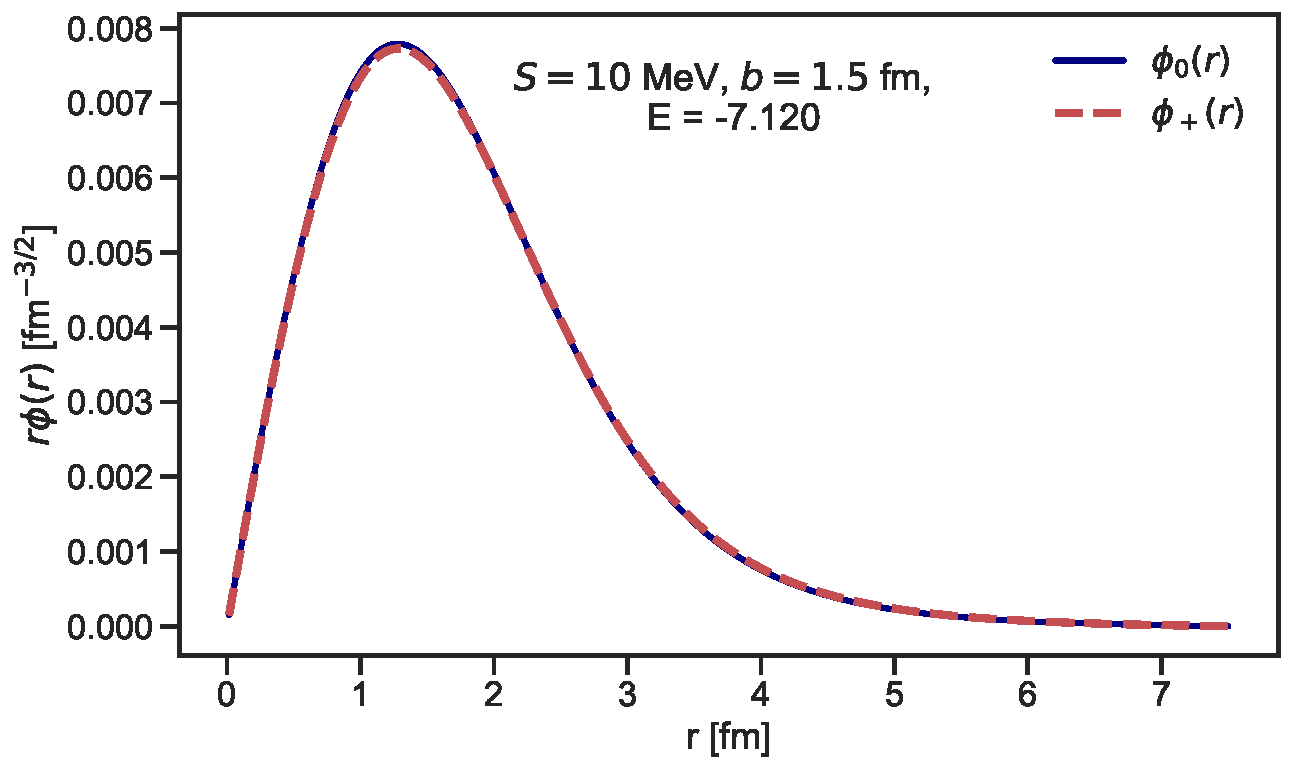
\includegraphics[width=\linewidth]{Figures/Integralplot_CoupledSystem.pdf}
    \end{sidecaption}
\end{figure}
Compared to \ref{fig:integralplot} the difference is negligible even accounting for the mass difference for the pions and nucleons ($m_N, m_P$). This means we can to a good estimation continue using only one pion wave function in our nuclear model. 